\documentclass[conference]{IEEEtran}
\IEEEoverridecommandlockouts

\usepackage[utf8]{inputenc}
\usepackage[T1]{fontenc}
\usepackage{cite}
\usepackage{amsmath,amssymb,amsfonts}
\usepackage{algorithmic}
\usepackage{algorithm}
\usepackage{graphicx}
\usepackage{textcomp}
\usepackage{subcaption} 
\usepackage{tabularx}
\usepackage{booktabs} 
% \usepackage{float}  
\usepackage{booktabs}     
\usepackage{xcolor}
\usepackage{textcomp}
\usepackage{xurl} 
\usepackage{array}
\renewcommand{\arraystretch}{1.2}
\usepackage{listings} 
\lstdefinestyle{ieeelisting}{
	basicstyle=\ttfamily\footnotesize,
    frame=single,
    breaklines=true,
    numbers=none,
    showstringspaces=false,
    columns=fullflexible
	}
\usepackage{acronym}
\newacro{ai}[AI]{Artificial Intelligence}
\newacro{ann}[ANN]{Artificial Neural Networks}
\newacro{dl}[DL]{Deep Learning}
\newacro{ml}[ML]{Machine Learning}
\newacro{cv}[CV]{Computer Vision}
\newacro{cnn}[CNN]{Convolutional Neural Network}
\newacro{dcnn}[DCNN]{Deep Convolutional Neural Network}
\newacro{svm}[SVM]{Support Vector Machine}
\newacro{se}[SE]{Squeeze-and-Excitation}
\newacro{map}[mAP]{Mean Average Precision}
\newacro{vit}[ViT]{Vision Transormer}
\newacro{yolo}[YOLO]{You Look Only Once}
\newacro{fpn}[FPN]{Feature Pyramid Network}
\newacro{iou}[IoU]{Intersection over Union}
\newacro{gradcam}[Grad-CAM]{Gradient-weighted Class Activation Mapping}

\usepackage[colorlinks=true, allcolors=blue]{hyperref} 
\def\BibTeX{{\rm B\kern-.05em{\sc i\kern-.025em b}\kern-.08em
    T\kern-.1667em\lower.7ex\hbox{E}\kern-.125emX}}
\begin{document}

\title{SEPierceStageNet: EfficientNet with SE-Attention for Grapevine Pierce’s Disease Stage Classification}

\author{\IEEEauthorblockN{1\textsuperscript{st} Sehrish Noreen}
\IEEEauthorblockA{\textit{dept. name of organization (of Aff.)} \\
\textit{name of organization (of Aff.)}\\
City, Country \\
email address or ORCID}
\and
\IEEEauthorblockN{2\textsuperscript{nd} Given Name Surname}
\IEEEauthorblockA{\textit{dept. name of organization (of Aff.)} \\
\textit{name of organization (of Aff.)}\\
City, Country \\
email address or ORCID}
\and
\IEEEauthorblockN{3\textsuperscript{rd} Given Name Surname}
\IEEEauthorblockA{\textit{dept. name of organization (of Aff.)} \\
\textit{name of organization (of Aff.)}\\
City, Country \\
email address or ORCID}
\and
\IEEEauthorblockN{4\textsuperscript{th} Given Name Surname}
\IEEEauthorblockA{\textit{dept. name of organization (of Aff.)} \\
\textit{name of organization (of Aff.)}\\
City, Country \\
email address or ORCID}
\and
\IEEEauthorblockN{5\textsuperscript{th} Given Name Surname}
\IEEEauthorblockA{\textit{dept. name of organization (of Aff.)} \\
\textit{name of organization (of Aff.)}\\
City, Country \\
email address or ORCID}
\and
\IEEEauthorblockN{6\textsuperscript{th} Given Name Surname}
\IEEEauthorblockA{\textit{dept. name of organization (of Aff.)} \\
\textit{name of organization (of Aff.)}\\
City, Country \\
email address or ORCID}
}

\maketitle

\begin{abstract}
Pierce's Disease is a becterial disease caused by Xylella fastidiosa. It affects the grapevine leaves. Accurate assessment of grapevine leaf health is important for precision agriculture. But traditional manual inspection is higly subjective and often inconsistent. Recent advances in \ac{dl} have enabled automated analysis of grapevine leaves. In this paper, we propose \textit{SEPierceStageNet}, a transfer learning model optimized for the multi-stage grapevine Pierce's Disease classification on a relatively small dataset. The model uses an \textit{EfficientNet-B0} backbone, enhanced with a \ac{se} attention module, and a compact classification head. It effectively extracts grapevine leaves feature for a better classification of disease stage. Our model achieves a training accuracy of 95.57\%, validation accuracy of 92.25\% and a test accuracy of 95.26\%, significantly outperforming baseline \textit{EfficientNet-B0} with 73.07\% and \textit{ResNet50} with 65.34\% test accuracy. These results highlight the model's potential to facilitate timely disease detection. It bridges the gap between baseline research models and practical precision agriculture applications.
\end{abstract}

\begin{IEEEkeywords}
Deep Learning, Computer Vision, Grapevine, Pierce Disease, EfficientNet, SE Attention
\end{IEEEkeywords}

\begin{figure*}[htbp]
\centerline{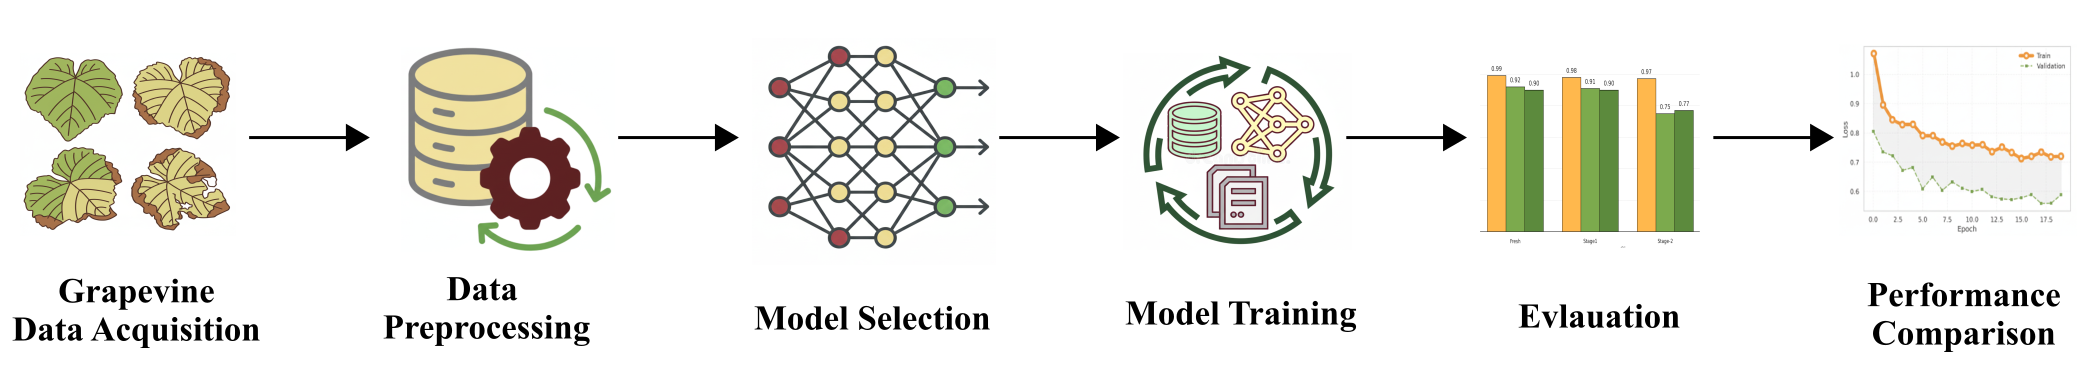
\includegraphics[width=\textwidth]{images/methodology.png}}
	\caption{Methodology of the proposed SEPierceStageNet: grapevine disease stage classification framework.}
	\label{fig:methodology}
\end{figure*}

\section{Introduction}
Pierce's Disease in grapevines is a fatal disease caused by the bacterium Xylella fastidiosa. This becterium hat lives in the xylem of grapevines. It blocks water flow and causes symptoms like leaf scorch, wilting, and eventual vine death. It spreads by insects like the \textit{Glassy Winged Sharpshooter}. Grapevine health and fruit quality are critical measures of vineyard productivity and quality. 
Recent climate studies indicate an increasing global risk of grapevine Pierce’s disease. Analyses of over 100,000 vineyards show that the area at risk in Europe has increased from 22\% to over 41\%. While in South Africa it has increased from roughly 6\% to more than 47\% \cite{GimenezRomero2025}. Global warming may also cause the spread of Pierce’s disease  into major European wine growing regions \cite{GimenezRomero2024}.

Making early disease detection and accurate assessment of leaf conditions is essential for precision viticulture Traditionally, plant leaf disease monitoring has been done through manual inspection. Manual inspection relies completely on human observation. Different inspectors may interpret the same symptoms in different ways that leads to inconsistent conclusions about leaf health. Traditional evaluation methods do not follow any uniform standard measure. These methods are also very time consuming. Only a small part of the vineyard can be examined manually due to resource constraints.

Recent advances in \ac{cv} and \ac{dl} have transformed this domain by enabling automated analysis of grapevine leaves through high resolution images. In particular, \ac{dl} models like \ac{cnn}s, have showed rreliable performance in detecting and classifying morphological and spectral patterns associated with leaf health and disease/ripeness stages. Existing studies highlight the efficiency of \ac{cv} approaches. \ac{cnn} classification models have achieved high accuracies.  Despite these advancements, many challenges remain. Most existing models are either computationally intensive or rely on large datasets. This limits their applicability in small vineyards. Many studies focus only on binary disease detection or single-stage ripening classification. Neglecting the nuanced multi-stage progression of grapevine leaves disease. Real-time deployability and lightweight architectures suitable for edge devices are rarely addressed, leaving a gap between research and practical vineyard implementation. 

To address these gaps, this paper proposes \textit{SEPierceStageNet}, a transfer learning model optimized for multi-stage grapevine leaf Pierce's Disease classification on a relatively small dataset. The model uses a frozen \textit{EfficientNet-B0} \cite{pmlr-v97-tan19a} backbone with selective feature extraction. It is enhanced by a lightweight \ac{se} attention \cite{Hu_2018_CVPR} module, and a compact classification head. By fine-tuning only a subset of the \textit{EfficientNet-B0} parameters, \textit{SEPierceStageNet} achieves accuracy of approximately 95\%. While  also maintained a low computational cost, making it suitable for real-time vineyard applications on edge devices. The key contributions of this paper include:
\begin{itemize}
    \item A multi-stage grapevine leaf Pierce's Disease classification model.
    \item Integration of a \ac{se} attention mechanism to enhance feature representation and improve stage wise disease classification accuracy.
    \item Robust performance on training, validation, and test splits, achieving a high accuracy on all splits that indicates generalizability to unseen data.
\end{itemize}

The rest of the paper is structured as follows. Section \ref{sec:rw} reviews most recent and relevant literature on grapevine leaf disease detection, including \ac{dl} architectures, attention mechanisms, and classical machine learning approaches. Section \ref{sec:methodology} details the materials and methods, covering dataset description, preprocessing pipelines, model architecture, and training strategy. Section \ref{sec:results} presents experimental results, performance evaluation. Section \ref{sec:comparison} comparative analysis with baseline pretrained models. Seciton \ref{sec:limitations} provides limitations, and directions for future work. Finally, Section \ref{sec:con} concludes the paper with key findings.

\section{Related Work}
\label{sec:rw}
Grapevine leaf disease detection has seen significant progress over the past decade. Advancements in \ac{dl}, \ac{ml}, and spectroscopic analysis. Among all, \ac{cnn}s have emerged as the most effective approach withh their capability of extracting spatial, textural, and morphological features from complex leaf images. For instance, \cite{Malagol2025} applied a ResNet based architecture to quantify hair structures on grape leaves with an accuracy of 95.41\%. Other than classification, segmentation of diseased regions has also been explored to focus on biologically relevant features only. Study \cite{Zhang2024GMamba} used a UNet state space model on PlantVillage dataset, achieving an \ac{iou} of 3.28. Object detection methods have also facilitated the on-field applications by enabling automated identification of diseased areas in leafs. \cite{Khan2025YOLOv7} reported a \ac{map} of 64.6\%, while a more recent YOLOv11 approach \cite{Zhou2025YOLOGrape} improved detection performance with a \ac{map} of 95.2\%.

Classification tasks have also reached strong levels of performance. ResNet models have showed stable and consistent behavior, \cite{Sagar2025} achieved 95\% accuracy on grape leaf datasets. Methods that fuse several backbone networks have further improved accuracy by using feature information from different architectures. For example, \cite{Vo2026AFCNet} combined \textit{ResNet50}, EfficientNetB0, and MobileNetV2, resulting in 99.83\% accuracy. Which shows that the use of different feature extractors together can enhance classification accuracy. Models that integrate transformer architectures with convolutional layers have also shown reliable results \cite{Zhang2025Transformer} gained 98.48\% accuracy. Similarly, cascaded \ac{cnn} models, as proposed by \cite{AlNasseri2025}; approached near perfect classification with 100\% accuracy. Efficient and compact models designed for faster inference have gained significant attention for edge devices. MobileNetV2 combined with\ac{vit} modules \cite{Tanvir2025} had strong outcomes with 99.2\% accuracy. While comparative evaluations \cite{Mathew2025} reported 99.5\% accuracy. \ac{dcnn} based on VGG16 \cite{Prasad2024} reached 99.18\% accuracy. Showing that classical architectures can still offer competitive performance. Modified \ac{cnn} models have further strengthened classification tasks, study \cite{Talaat2025} reported 99.7\% accuracy and \cite{Karim2024} reached 99.66\%. Even simpler refined \ac{cnn} approaches \cite{Naik2025} have stable and dependable performance across multiple grape leaf disease datasets.

Beyond \ac{dl} methods, classical \ac{ml} methods also provide complementary insights that are reliable for nutrient assessment and early pathogen detection. \ac{svm}s combined with feature optimization  were applied by \cite{Shi2025} to classify fungal spores. They report 97.5\% accuracy, highlighting the usefulness of traditional \ac{ml} techniques when paired with domain specific feature engineering. Chemometric regression models have been successfully used for predicting macro and micro-nutrient concentrations, \cite{Manzano2025} reported an R² of 0.90 for sodium content. Early detection of viral infections has been made possible through hyperspectral and multispectral sensing techniques. As presented in paper \cite{Lee2024} where strong infections were identified at CT values below 35.

These studies show that combining \ac{cnn}, hybrid transformers, multi-backbone fusion, and feature based \ac{ml} provides accurate solutions for grape leaf disease detection, nutrient assessment, and pathogen monitoring. Edge deployable models with explainable AI techniques like \ac{gradcam} enable practical precision viticulture. They support the rapid disease assessment and optimized vineyard management. Spectroscopic and chemometric methods complement imaging for non destructive plant health monitoring.

\section{Material and Methods}
\label{sec:methodology}
This study implements a modified EfficientNetB0 \ac{dl} model for detecting and classifying Pierce's Disease stages in grapevine leaves. The methodology follows five steps: Data acquisition, Preprocessing, Classification and evaluation, Results analysis, and Comparative assessment as shown in Figure~\ref{fig:methodology}. The complete pipeline was implemented in Python. We used PyTorch and executed model on Google Colab with GPU acceleration.

\subsection{Data Description}
The dataset consists of labeled images of grapevine leaves organized into four classes. Each class representing progressive stage of Pierce's Disease. The classification includes Fresh leaves, Stage 1 having early infection, Stage 2 with moderate progression, and Stage 3 is advanced infection in leaves. Figure~\ref{fig:datasamples} shows data samples from training subset. Images were sourced from the ``PierceDisease: Xylella fastidiosa affected Grape Leaves comprehensive image dataset'' \cite{Islam2025PierceDisease} dataset, which provides four progression stages of Pierce's Disease. We split dataset into Train, Test and Validaton subsets. The dataset contains 4,004 images in total. These images were distributed as: 3,203 training images, 400 validation images, and 401 test images. Table~\ref{tab:data_distribution} shows the data distribution. As shown in Listing~\ref{lst:classmapping}, a consistent integer mapping was established for standard label encoding across all subsets. 

\begin{table}[h!]
    \caption{Distribution of images across dataset splits for grapevine Pierce's Disease stages.}
    \centering
    \begin{tabular}{m{0.2\columnwidth} m{0.2\columnwidth} m{0.2\columnwidth} m{0.2\columnwidth}}
        \toprule
        \textbf{Stage} & \textbf{Train} & \textbf{Validation} & \textbf{Test} \\
        \midrule
        Fresh   & 800 & 100 & 100 \\
        Stage 1 & 800 & 100 & 100 \\
        Stage 2 & 800 & 100 & 100 \\
        Stage 3 & 803 & 100 & 101 \\
        \midrule
        \textbf{Total} & \textbf{3203} & \textbf{400} & \textbf{401} \\
        \bottomrule
    \end{tabular}
    \label{tab:data_distribution}
\end{table}

\begin{figure}[htbp]
	\centering
    \begin{subfigure}[b]{0.24\columnwidth}
		\centering
		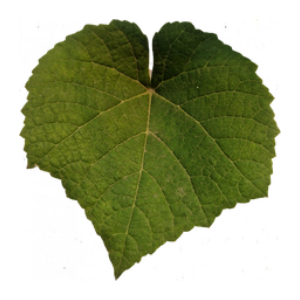
\includegraphics[width=\linewidth]{images/fresh.png} 
		\caption{Fresh Leaf}
		\label{fig:fresh}
	\end{subfigure}
    \begin{subfigure}[b]{0.24\columnwidth}
		\centering
		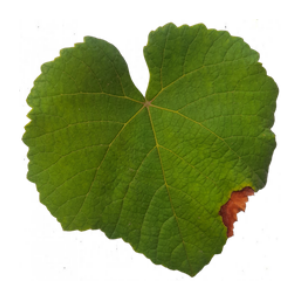
\includegraphics[width=\linewidth]{images/stage1.png} 
		\caption{Stage 1}
		\label{fig:stage1}
	\end{subfigure}
    \begin{subfigure}[b]{0.24\columnwidth}
		\centering
		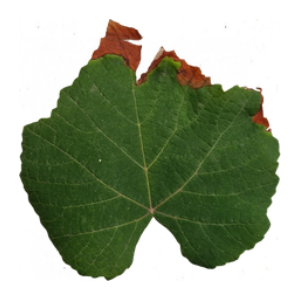
\includegraphics[width=\linewidth]{images/stage2.png} 
		\caption{Stage 2}
		\label{fig:stage2}
	\end{subfigure}
    \begin{subfigure}[b]{0.24\columnwidth}
		\centering
		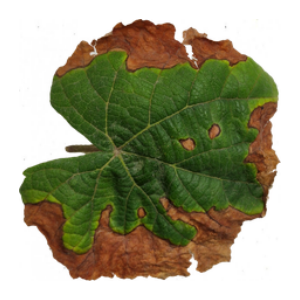
\includegraphics[width=\linewidth]{images/stage3.png} 
		\caption{Stage 3}
		\label{fig:stage3}
	\end{subfigure}
	\caption{Samples from Grapevine Pierce's Disease dataset.}
	\label{fig:datasamples}
\end{figure}

\begin{lstlisting}[style=ieeelisting, frame=none,
caption={Class mapping in code},
label={lst:classmapping}]
Class mapping: {'Fresh': 0, 'Stage1': 1, 'Stage-2': 2, 'Stage-3': 3}
Classes: ['Fresh', 'Stage1', 'Stage-2', 'Stage-3']
\end{lstlisting}

\subsection{Pre-processing}
Two different preprocessing pipelines were implemented. One for training with extensive data augmentation. Other for validation and testing with minimal transformations. Training subset transformations include resizing images to 224×224 px, random horizontal and vertical flipping, ±20-degree rotation, color jittering, random affine transformations, and ImageNet normalization. Validation and test subset transformations consisted only of resizing, tensor conversion, and normalization. All the transformations are applied during training, on the go.This strategy enhances model generalization and also maitains evaluation consistency. Figure~\ref{fig:preprocessing} shows some of preprocessing transformations.
\begin{figure}[htbp]
\centerline{
\includegraphics[width=0.9\columnwidth]{images/preprocessing.png}}
	\caption{Examples of data augmentation techniques applied during the training.}
	\label{fig:preprocessing}
\end{figure}

\subsection{Model Training and Evaluation}
The primary model, \textit{SEPierceStageNet}, is based on \textit{EfficientNet-B0}. It uses transfer learning. As shown in Algorithm~\ref{alg:SEPierceStageNet}, the architecture integrates a lightweight \ac{se} module to enhance feature discrimination. At the end is a custom classification head for final predictions. Figure~\ref{fig:model} illustrates the overall model structure. For benchmarking, standard \textit{EfficientNet-B0} and \textit{ResNet50} architectures were implemented under identical conditions.

\begin{figure*}[htbp]
\centerline{
\includegraphics[width=0.9\textwidth]{images/model.png}}
	\caption{Architecture of \textit{SEPierceStageNet} with \textit{EfficientNet-B0} backbone and \ac{se} attention.}
	\label{fig:model}
\end{figure*}

\begin{algorithm}
\caption{SEPierceStageNet Training, Validation, and Testing.}
\label{alg:SEPierceStageNet}
\begin{algorithmic}[1]
\STATE \textbf{Input:} Image batch $I$
\STATE \textbf{Output:} Predicted disease class labels

\STATE Load pretrained \textit{EfficientNet-B0} backbone
\STATE Freeze first six feature blocks
\STATE Insert SE attention module
\STATE Construct classifier head

\FOR{each training batch $I$}
    \STATE $x \gets \texttt{Backbone}(I)$
    \STATE $x \gets \texttt{SE}(x) \odot x$
    \STATE $y \gets \texttt{Classifier}(x)$
    \STATE Compute cross-entropy loss
    \STATE Update trainable parameters
\ENDFOR

\STATE Evaluate model on validation data
\STATE Evaluate model on test data
\STATE Return trained SEPierceStageNet model and test predictions
\end{algorithmic}
\end{algorithm}

\subsubsection{Backbone}
The backbone of the model is based on \textit{EfficientNet-B0}, which provides hierarchical feature extraction from input images. The model uses pretrained weights to retain generic visual features while also adapting to the target dataset. Approximately 75\% of the early layers were frozen (see Listing~\ref{lst:backbone}), allowing only the later layers to be fine-tuned. This strategy preserves robust low-level features learned from large-scale data while focusing computational resources on adapting higher-level representations to the specific characteristics of our dataset, improving convergence and reducing the risk of overfitting.

\begin{lstlisting}[style=ieeelisting, frame=none,
caption={Backbone Initialization of SEPierceStageNet},
label={lst:backbone}]
Initialize EfficientNet-B0 with pretrained ImageNet weights
Divide the backbone into ordered feature blocks
For each feature block with index i do
    If i < 6 then
        Freeze all parameters of the block
    Else
        Allow parameters to be updated during training
    End if
End for
\end{lstlisting}

\subsection{\ac{se} Module}

The \ac{se} module is designed to improve the representational power of a network by explicitly modeling channel-wise interdependencies. It consists of two main operations:

\begin{enumerate}
    \item \textbf{Squeeze:} Global average pooling is applied to each feature map to generate a channel-wise descriptor:
    \begin{equation}
        z_c = \frac{1}{H \times W} \sum_{i=1}^{H} \sum_{j=1}^{W} X_c(i,j)
    \end{equation}
    where \(X_c \in \mathbb{R}^{H \times W}\) is the \(c\)-th channel of the feature map, and \(z_c\) is its global descriptor.

    \item \textbf{Excitation:} The channel descriptors are passed through a small two-layer fully connected network with a non-linear activation and a sigmoid to generate channel-wise weights:
    \begin{equation}
        s = \sigma(W_2 \delta(W_1 z))
    \end{equation}
    where \(W_1\) and \(W_2\) are learnable weight matrices, \(\delta\) is the ReLU activation, and \(\sigma\) is the sigmoid function.
    
    \item \textbf{Recalibration:} Finally, the original feature maps are rescaled using these learned weights:
    \begin{equation}
        \tilde{X}_c = s_c \cdot X_c
    \end{equation}
\end{enumerate}

Although \textit{EfficientNet-B0} contains built-in \ac{se} blocks, we introduce an additional trainable \ac{se} module at the feature head to better adapt to our dataset. This module performs task-specific channel recalibration on the final convolutional features, enhancing validation accuracy while maintaining a small train–validation gap. Adding this lightweight module avoids unfreezing more backbone layers, which could increase overfitting, yet provides effective channel-level feature refinement with minimal parameter overhead (see Section~\ref{sec:results}).


\begin{lstlisting}[style=ieeelisting, frame=none,
caption={\ac{se} Module},
label={lst:semodule}]
Input: Feature map F (1280 channels)

Global average pool F
Reduce channels to 1280/16, apply ReLU, restore to 1280
Apply sigmoid and scale F by attention weights

Output: Recalibrated feature map
\end{lstlisting}

\subsubsection{Classification Head}
The last part is classification head. It maps the attended feature maps to final predictions. It includes a fully connected layer, ReLU activation, dropout for regularization. At last, a final linear layer for the outputs corresponding to the target classes. Given in Listing~\ref{{lst:classhead}}.

\begin{lstlisting}[style=ieeelisting, frame=none, basicstyle=\ttfamily, caption={Classification Head}, label={lst:classhead}]
Input: Feature map F

Apply global average pooling and flatten
Fully connected layer with 512 units, ReLU activation, and dropout
Fully connected layer to output class scores

Output: Class scores
\end{lstlisting}

\subsubsection{Forward Pass}
During the forward pass, the input images first pass through the backbone to extract feature maps. Then \ac{se} module computes channel-wise attention and scales the features. Finally, the classification head processes those features and gives the class predictions. Shown in Listing~\ref{{lst:fpass}}.

\begin{lstlisting}[style=ieeelisting, frame=none,
caption={Forward Pass of SEPierceStageNet},
label={lst:fpass}]
Input: Image batch X

Extract features using EfficientNet-B0 backbone
Apply SE module and reweight features with attention
Pass features through classification head

Output: Class predictions
\end{lstlisting}

\subsubsection{Device Setup and Model Summary}
The model is initialized and moved to the available GPU device. We used google colab. A summary of the network is generated to visualize layer dimensions and parameters.

\subsection{Evaluation Metrics}
Model performance was assessed using standard classification metrics accuracy, precision, recall and f1-score. The macro-averaging approach was used to give equal weight to all classes.

\begin{itemize}
    \item \textbf{Accuracy}: Proportion of correct predictions out of all predictions of model:
    \begin{equation}
        \text{Accuracy} = \frac{1}{N} \sum_{i=1}^{N} \frac{TP_i + TN_i}{TP_i + TN_i + FP_i + FN_i}
    \end{equation}

    \item \textbf{Precision}: Measure how many positive predictions of model are actually correct:
    \begin{equation}
        \text{Precision} = \frac{1}{N} \sum_{i=1}^{N} \frac{TP_i}{TP_i + FP_i}
    \end{equation}

    \item \textbf{Recall}: Ratio of correctly predicted positive samples to all actual positive samples:
    \begin{equation}
        \text{Recall} = \frac{1}{N} \sum_{i=1}^{N} \frac{TP_i}{TP_i + FN_i}
    \end{equation}

    \item \textbf{F1-Score}: Harmonic mean of precision and recall for each class:
    \begin{equation}
        \text{F1-Score} = \frac{1}{N} \sum_{i=1}^{N} \frac{2 \cdot \text{Precision}_i \cdot \text{Recall}_i}{\text{Precision}_i + \text{Recall}_i}
    \end{equation}
\end{itemize}

In addition to this, onfusion matrix was also visualized to analyze misclassification patterns. Per-class classification reports generated to provide detailed performance across all disease stages. These statistics are given in Section~\ref{sec:results}.

\begin{figure*}[!t]
    \centering

    % row1
    \begin{subfigure}[b]{0.45\textwidth}
        \centering
        
\includegraphics[width=\linewidth]{images/accuracy_plot.png}
        \caption{Accuracy}
        \label{fig:accuracy}
    \end{subfigure}
    \begin{subfigure}[b]{0.45\textwidth}
        \centering
        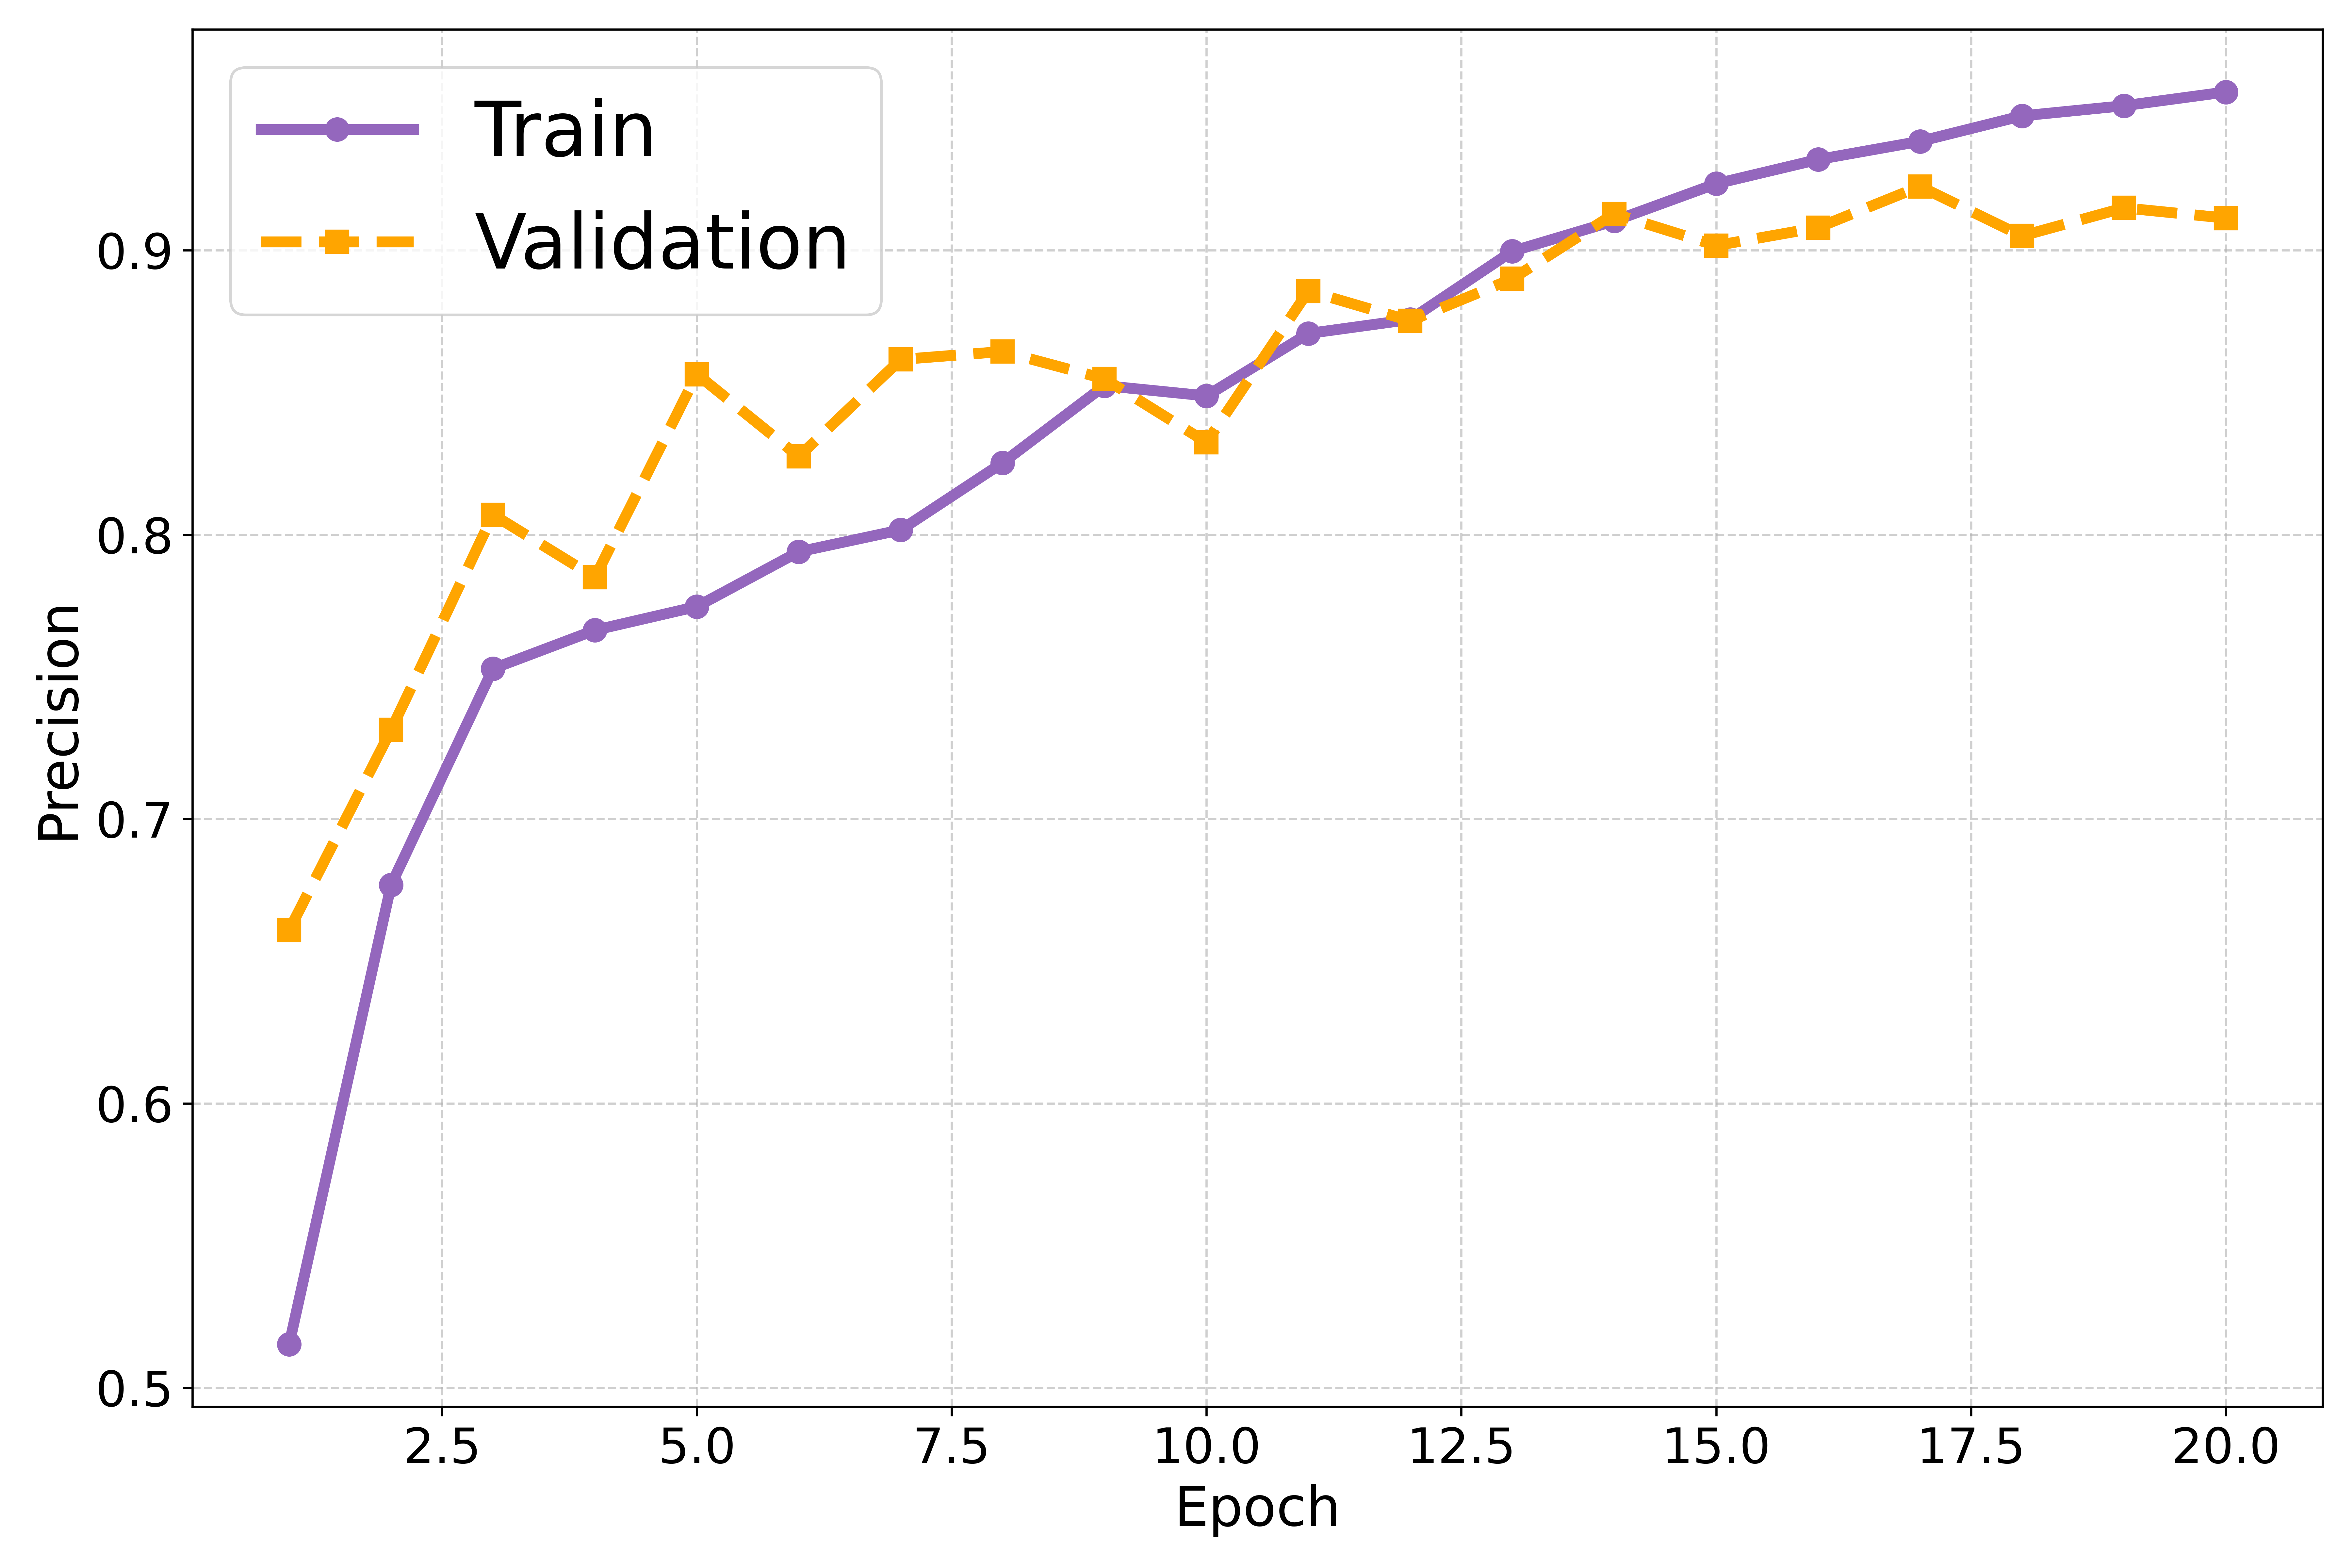
\includegraphics[width=\linewidth]{images/precision_plot.png}
        \caption{Precision}
        \label{fig:precision}
    \end{subfigure}

    \vspace{0.5em}

    % row2
    \begin{subfigure}[b]{0.45\textwidth}
        \centering
        
\includegraphics[width=\linewidth]{images/recall_plot.png}
        \caption{Recall}
        \label{fig:recall}
    \end{subfigure}
    \begin{subfigure}[b]{0.45\textwidth}
        \centering
        
\includegraphics[width=\linewidth]{images/f1_plot.png}
        \caption{F1-score}
        \label{fig:f1}
    \end{subfigure}

    \caption{Training and validation curves for \textit{SEPierceStageNet}.}
    \label{fig:performance}
\end{figure*}

\section{Results}
\label{sec:results}
\textit{SEPierceStageNet} demonstrated strong and consistent performance on training, validation, and test datasets. It outperforms baseline architectures \textit{EfficientNet-B0} and ResNet-50. The model was trained for up to 20 epochs. We used an ImageNet pretrained \textit{EfficientNet-B0} backbone combined with an \ac{se} module, custom classification head, optimized using AdamW. The pretrained backbone was fine-tuned with a learning rate of $1\times10^{-4}$. The classifier trained at $1\times10^{-3}$.  Cross-entropy loss with label smoothing of 0.1 was applied. A OneCycle learning rate scheduler with a 40\% warm up period and cosine annealing was used. Mixed precision training accelerated computations and reduced the memory usage. We implemented Early stopping with a patience of 5 epochs to prevent overfitting. The best performing model based on validation accuracy was selected.

Training and validation metrics recorded for each epoch; including accuracy, precision, recall, and F1-score. The model showed steady improvements with an early training accuracy of 51.20\% and validation accuracy of 63.25\% after the first epoch. By epoch 10, training accuracy reached 84.86\% and validation accuracy 82.75\%, showing an effective learning. The final evaluation metrics are summarized in Table~\ref{tab:SEPierceStageNet_metrics}.

\begin{table}[H]
\caption{Training, validation, and test metrics of \textit{SEPierceStageNet}.}
\centering
\begin{tabular}{m{0.3\columnwidth} m{0.1\columnwidth} m{0.1\columnwidth} m{0.1\columnwidth} m{0.1\columnwidth}}
\toprule
\textbf{Dataset} & \textbf{Accuracy} & \textbf{Precision} & \textbf{Recall} & \textbf{F1 Score} \\
\midrule
Training Set & 0.9557 & 0.9556 & 0.9557 & 0.9556 \\
Validation Set & 0.9225 & 0.9224 & 0.9225 & 0.9222 \\
Test Set & 0.9526 & 0.9526 & 0.9525 & 0.9524 \\
\bottomrule
\end{tabular}
\label{tab:SEPierceStageNet_metrics}
\end{table}

The test results confirm that our model generalizes well on unseen data. It maintains high precision and recall on all disease stages. A total of 401 test samples were processed. It made 383 correct predictions and 18 misclassifications, resulting in an empirical test accuracy of 95.51\%. Correctly classified samples had high confidence ranging from 0.82 to 0.94. While misclassified samples had lower confidences. Random sample predictions are shown in Figure~\ref{fig:predictions}, showing the model's ability to diffirentiate between fresh, stage 1, stage 2, and stage 3 disease stages.

\begin{figure}[H]
\centerline{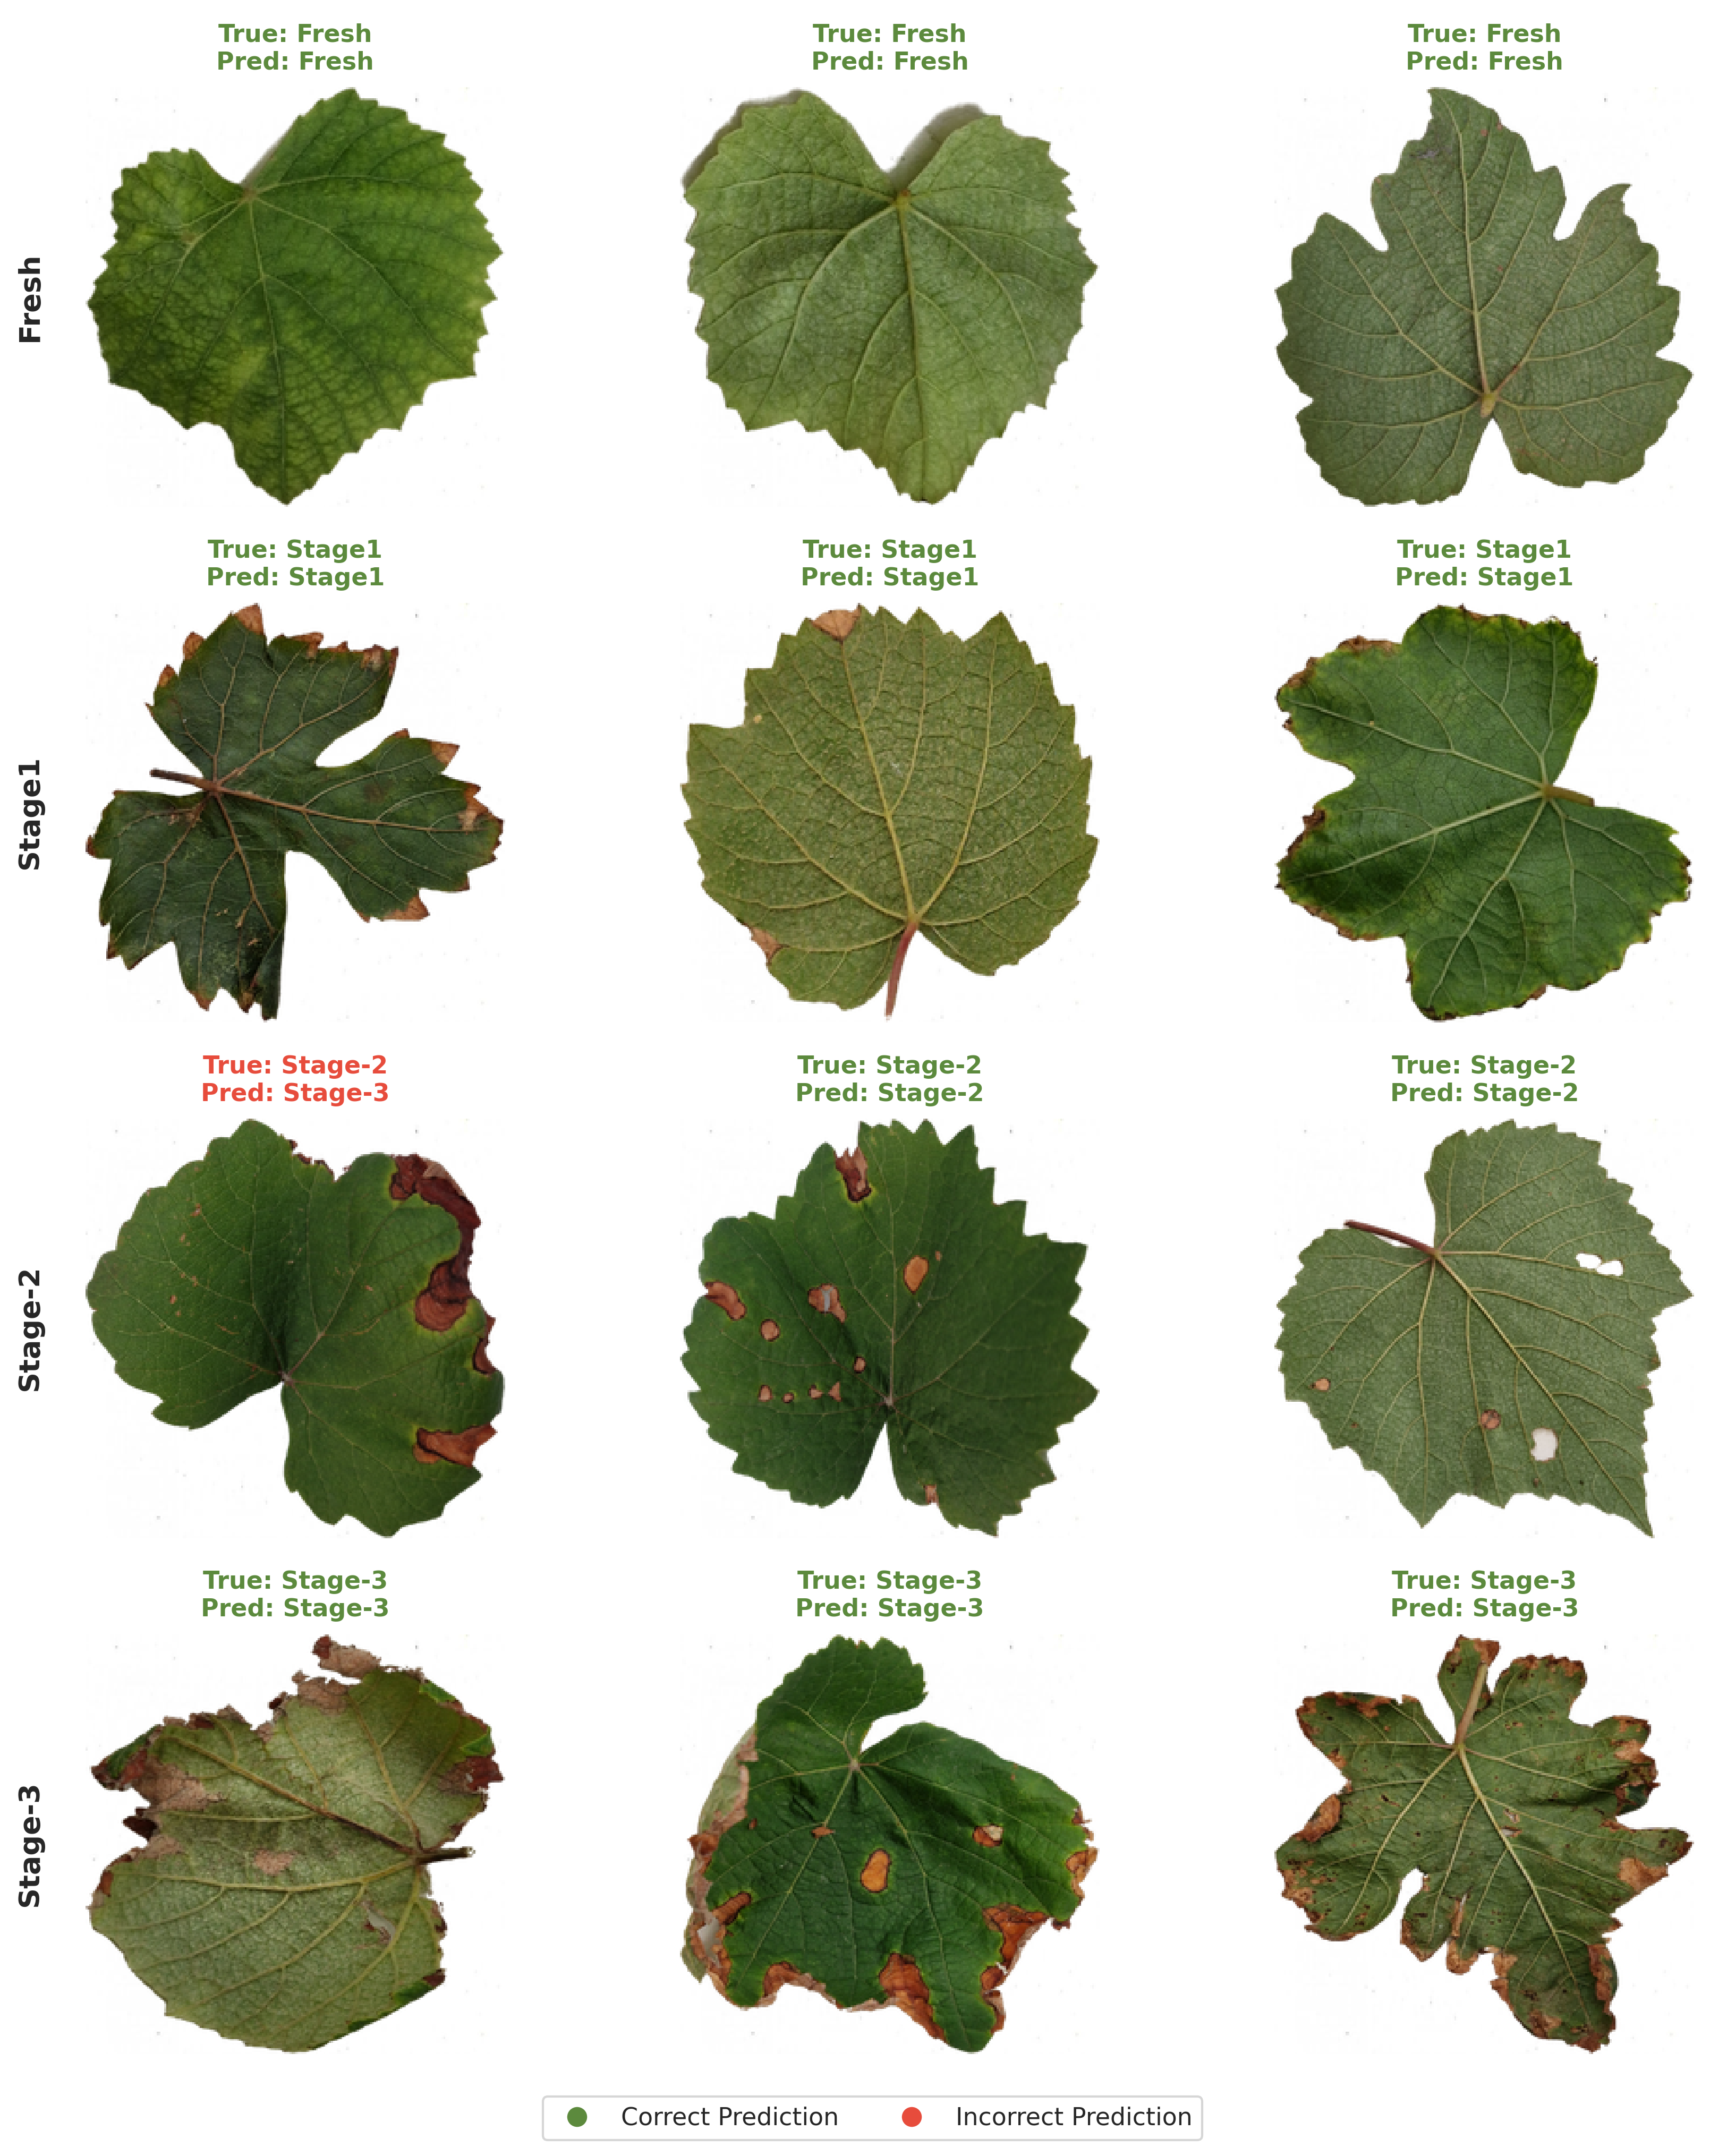
\includegraphics[width=\columnwidth]{images/test_samples_visualization.png}}
\caption{Prediction results of \textit{SEPierceStageNet} on the test subset. Correct classifications are indicated with green, misclassified samples are highlighted with red color.}
\label{fig:predictions}
\end{figure}

Class-wise evaluation indicates high accuracy across all disease stages. Small number of misclassifications occurred between similar disease stages: Stage 2 and Stage 3. So errors are systematic and are linked to visual similarities in these two stages not random predictions. Figure~\ref{fig:perclass} illustrates the accuracy of each class on training, validation, and test sets, showing a stable performance in all classes.

\begin{figure}[H]
\centerline{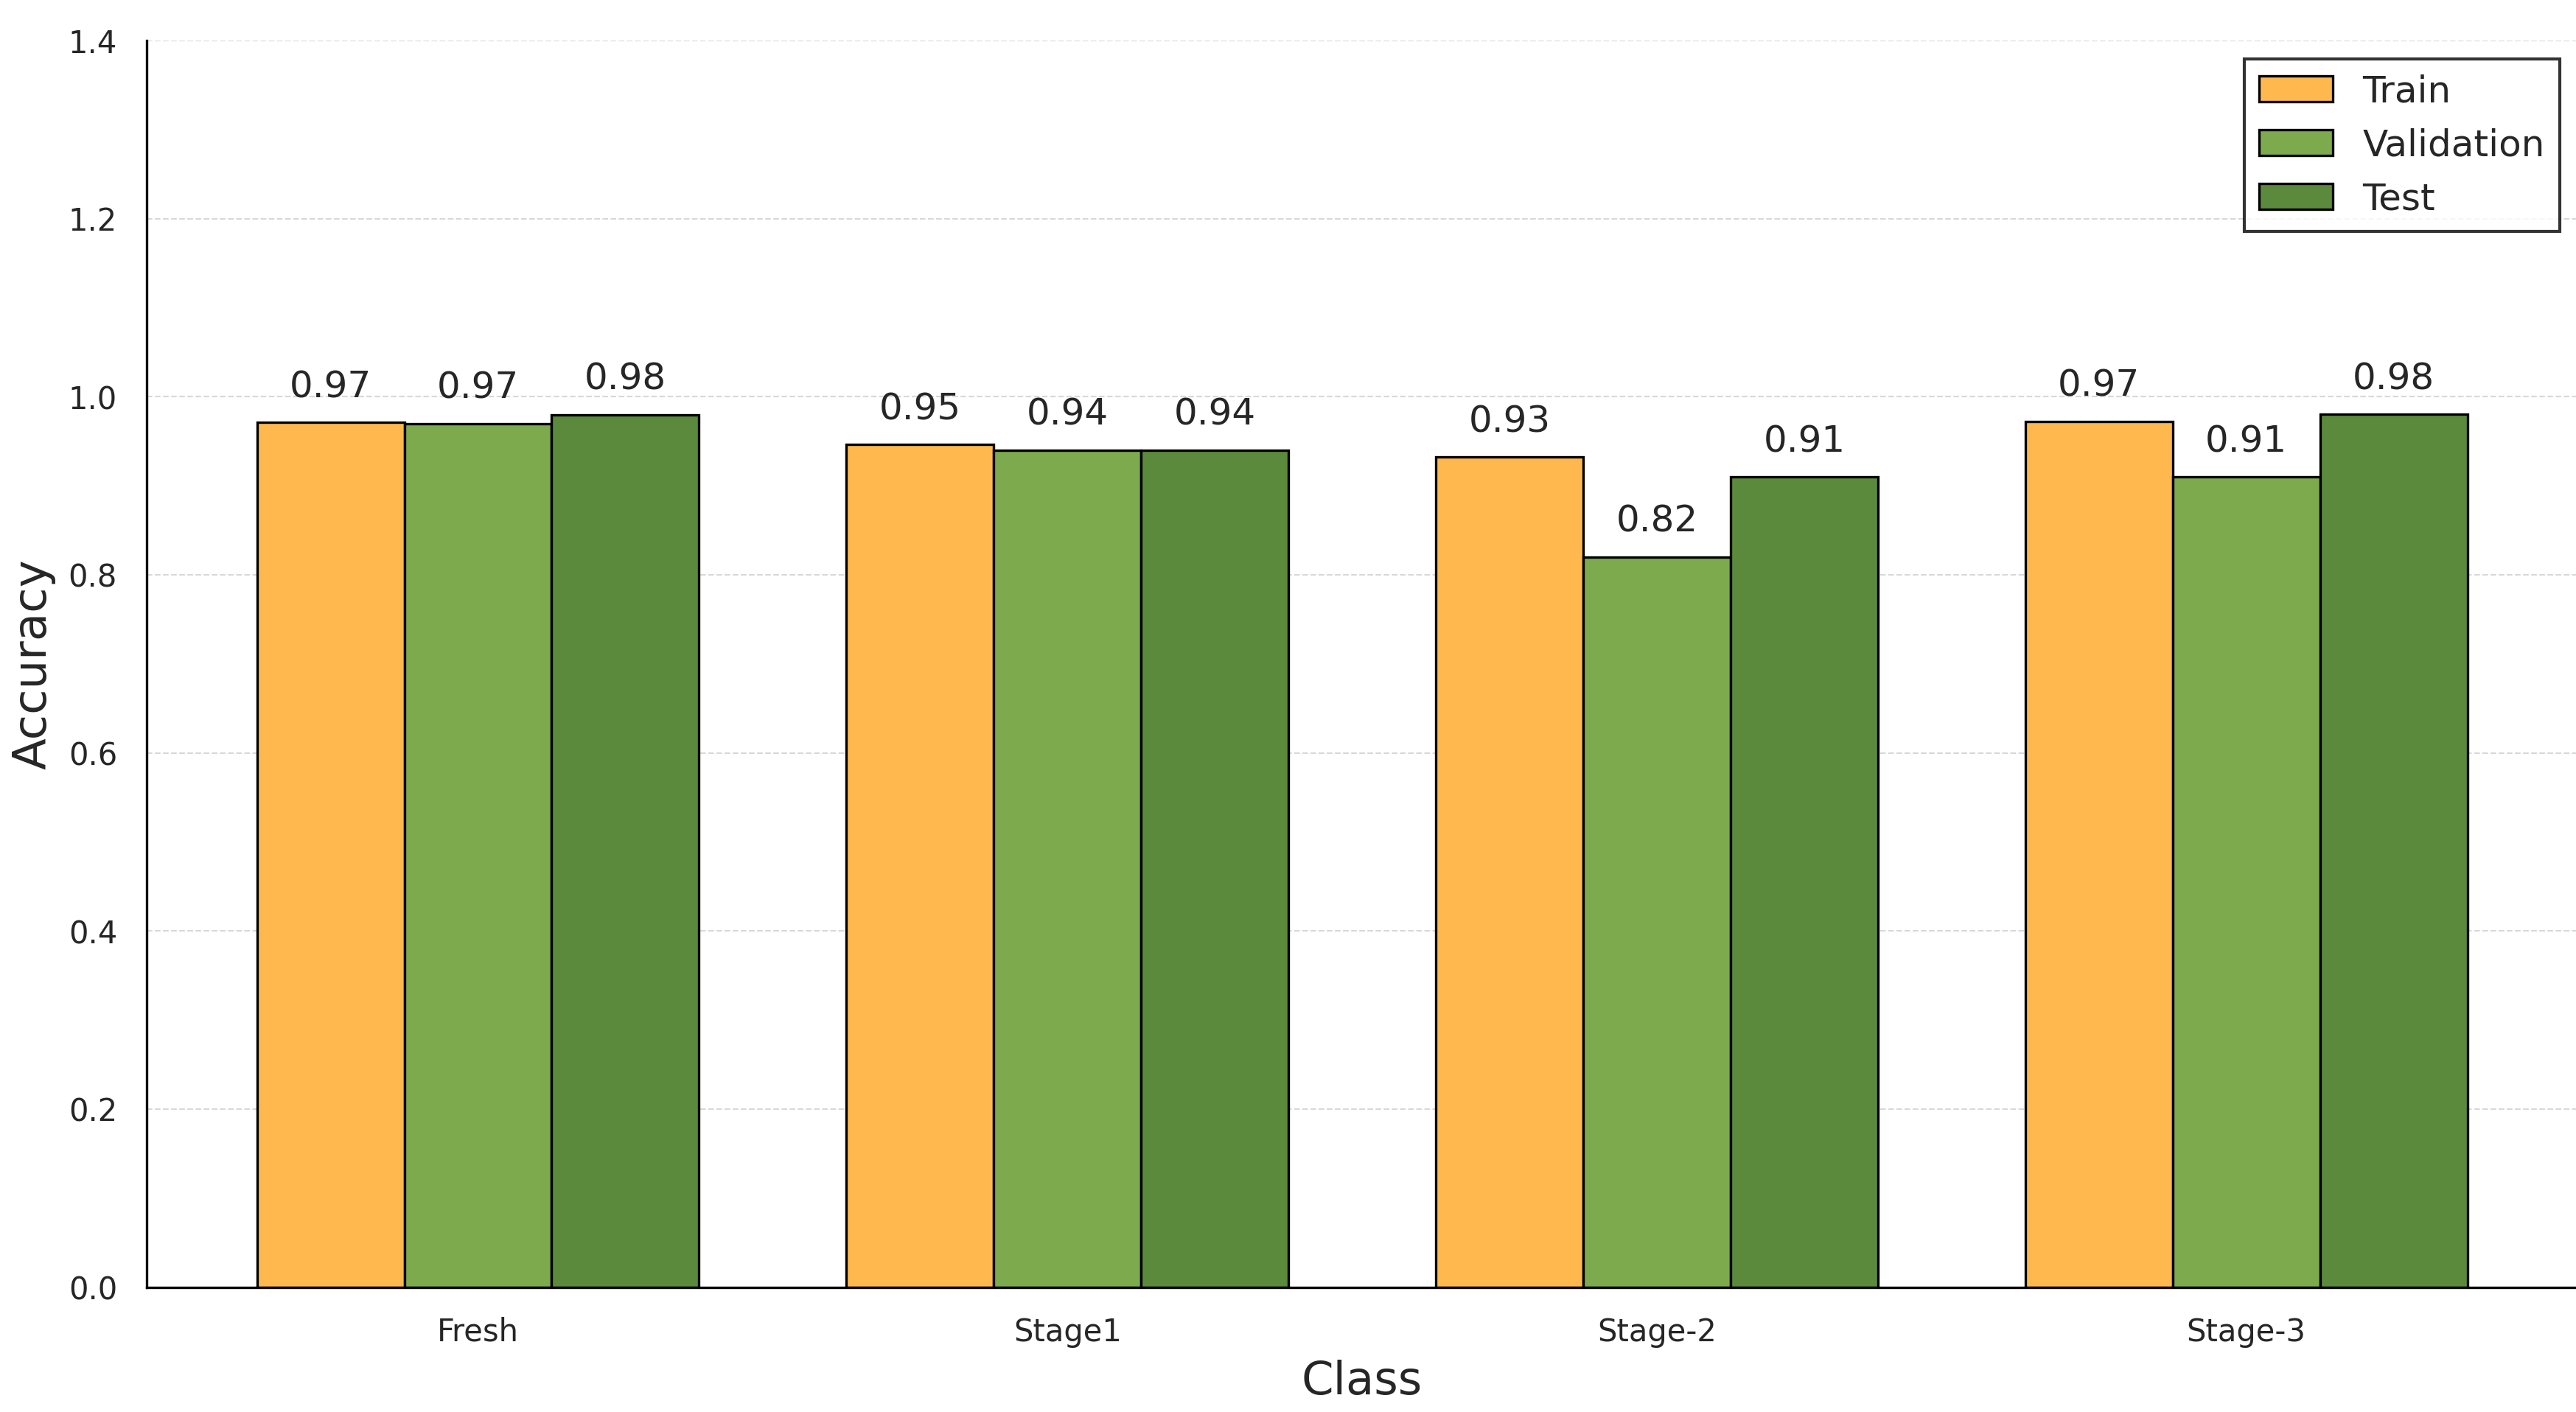
\includegraphics[width=\columnwidth]{images/per_class_accuracy_all_sets.png}}
\caption{Class-wise accuracy of proposed model on training, validation, and test datasets.}
\label{fig:perclass}
\end{figure}

The confusion matrix for the test set given in Figure~\ref{fig:cmatrix} provides insights into misclassifications between adjacent disease stages. Supporting the claim that errors are primarily due to visual resemblance rather than random noise. This reveals the model's logical performance in disease stage classification.

\begin{figure}[H]
\centerline{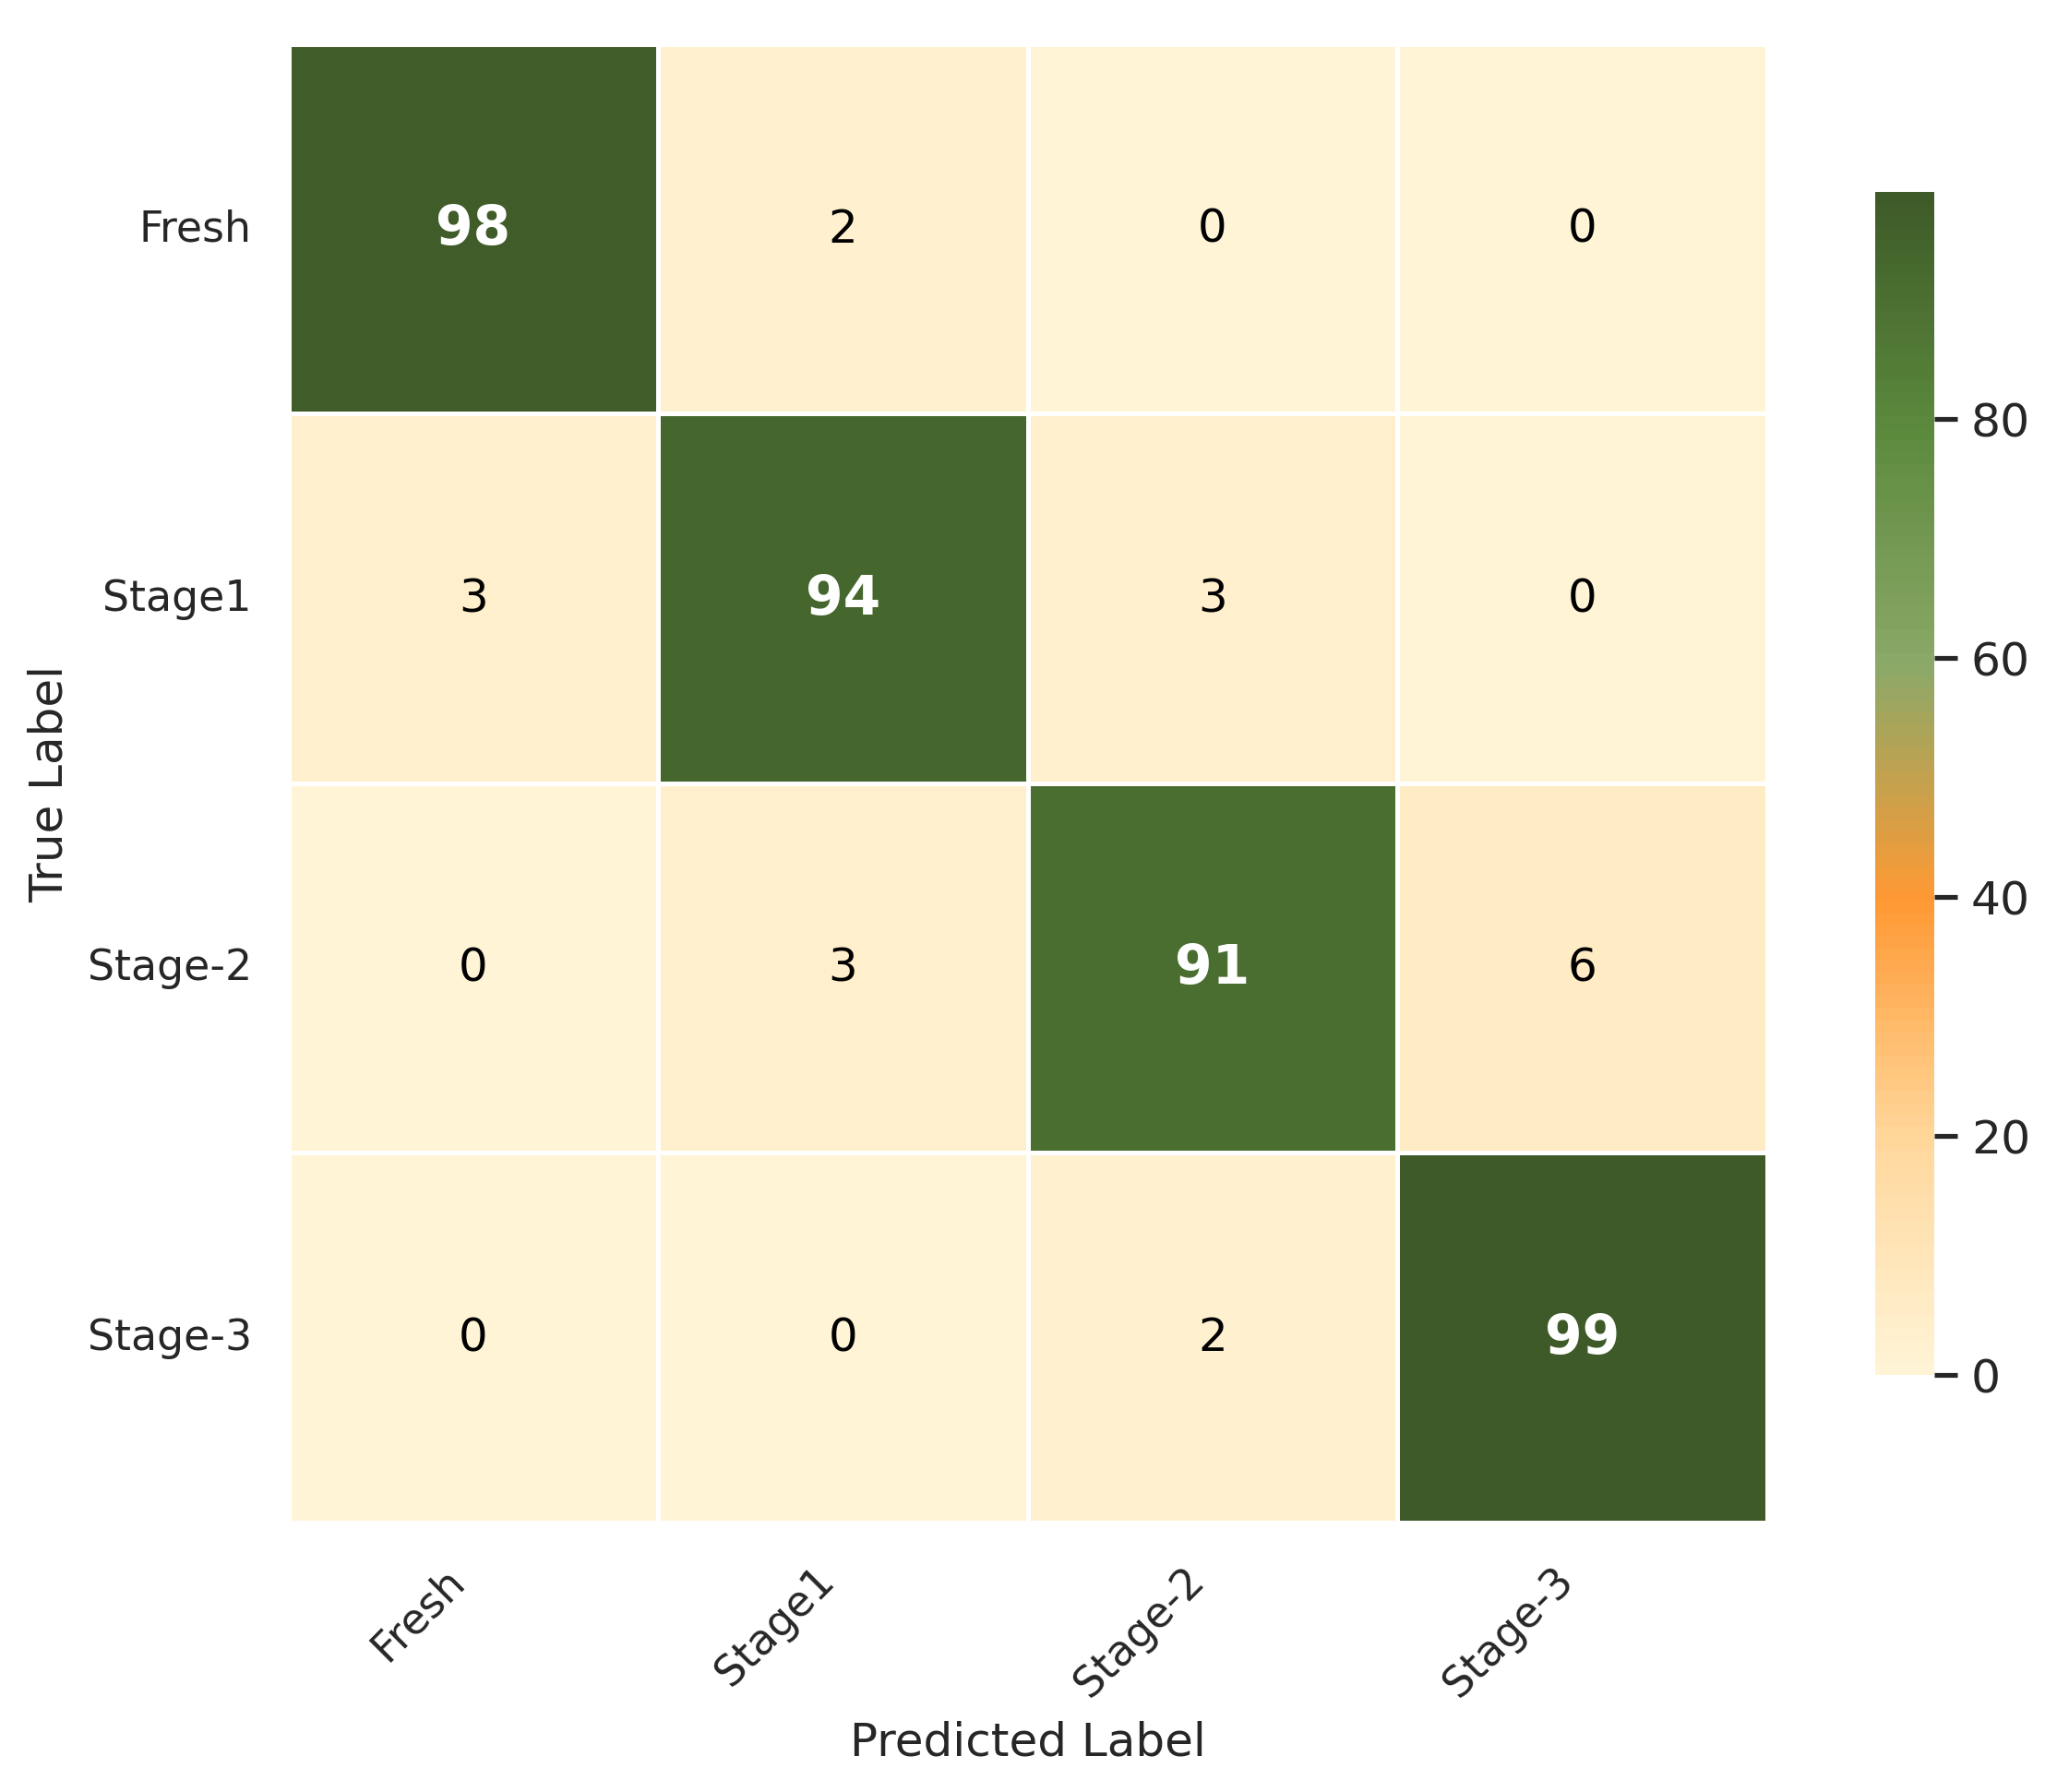
\includegraphics[width=0.9\columnwidth]{images/confusion_matrix_test.png}}
\caption{Confusion matrix for the test dataset with true and predicted class labels.}
\label{fig:cmatrix}
\end{figure}

Overall, the model has reliable performance for grapevine disease stage classification. Given a high accuracy, precision, recall, and F1-scores across all subsets.

\begin{table*}[!t]
\caption{Performance Comparison of \textit{SEPierceStageNet} and pretrained Baseline Models on Training, Validation, and Test Sets; Training accuracy is of the best validation epoch.}
\centering
\begin{tabular}{
m{0.30\textwidth}
m{0.10\textwidth}
m{0.10\textwidth}
m{0.10\textwidth}
m{0.15\textwidth}
}
\toprule
\textbf{Model} &
\textbf{Train Acc.} &
\textbf{Val Acc.} &
\textbf{Test Acc.} &
\textbf{Params (M)} \\
\midrule

\textbf{\textit{SEPierceStageNet}} &
\textbf{0.9557} &
\textbf{0.9225} &
\textbf{0.9526} &
\textbf{6.16 (2.19 Trainable)} \\

\textit{EfficientNet-B0} &
0.6712 &
0.7825 &
0.7307 &
5.30 \\

\textit{ResNet50} &
0.6254 &
0.7325 &
0.6534 &
25.60 \\

\bottomrule
\end{tabular}
\label{tab:model_comparison}
\end{table*}

\section{Model Comparison and Analysis}
\label{sec:comparison}
To assess the effectiveness of \textit{SEPierceStageNet}, we made a comparison with two widely used baseline models: \textit{EfficientNet-B0} and \textit{ResNet50}. Both baseline models were trained in same conditions as \textit{SEPierceStageNet}. We used ImageNet pretrained weights, the AdamW optimizer, and a similar training schedule for up to 20 epochs on the same training and validation subsets. Detailed comparison given in Table~\ref{tab:model_comparison}.

The final test results indicate that \textit{SEPierceStageNet} outperforms both baseline pretrained models. \textit{EfficientNet-B0} had a test accuracy of 73.07\% with precision 0.7290, recall 0.7307, and F1-score 0.7261. \textit{ResNet50} had 65.34\% accuracy with precision 0.6816, recall 0.6534, and F1-score 0.6563. In contrast, \textit{SEPierceStageNet} had 95.26\% accuracy, 0.9526 precision, 0.9525 recall, and 0.9524 F1-score. Outperforming both pretrained models in faster learning and superior generalization.

Figures~\ref{fig:eb} and \ref{fig:resnet} provide the validation accuracy and loss curves for \textit{EfficientNet-B0} and \textit{ResNet50}. \textit{EfficientNet-B0} reached its highest validation accuracy of 78.25\% at epoch 14. \textit{ResNet50} peaked at 73.25\% at epoch 11. These trends show the slower convergence of these models and lower overall performance as compared to \textit{SEPierceStageNet}, which achieved a best validation accuracy of 92.25\% at 17 epoch.

The baseline EfficientNet-B0 exhibits limited generalization, with validation accuracy saturating at ~78\%. The proposed \ac{se} module acts as a task specific attention adapter applied to the final feature representation. This enables domain aware channel recalibration under partial freezing. This results in validation accuracy improvement of ~14\% and a reduced training and validation gap.

\begin{figure*}[!t]
    \centering
    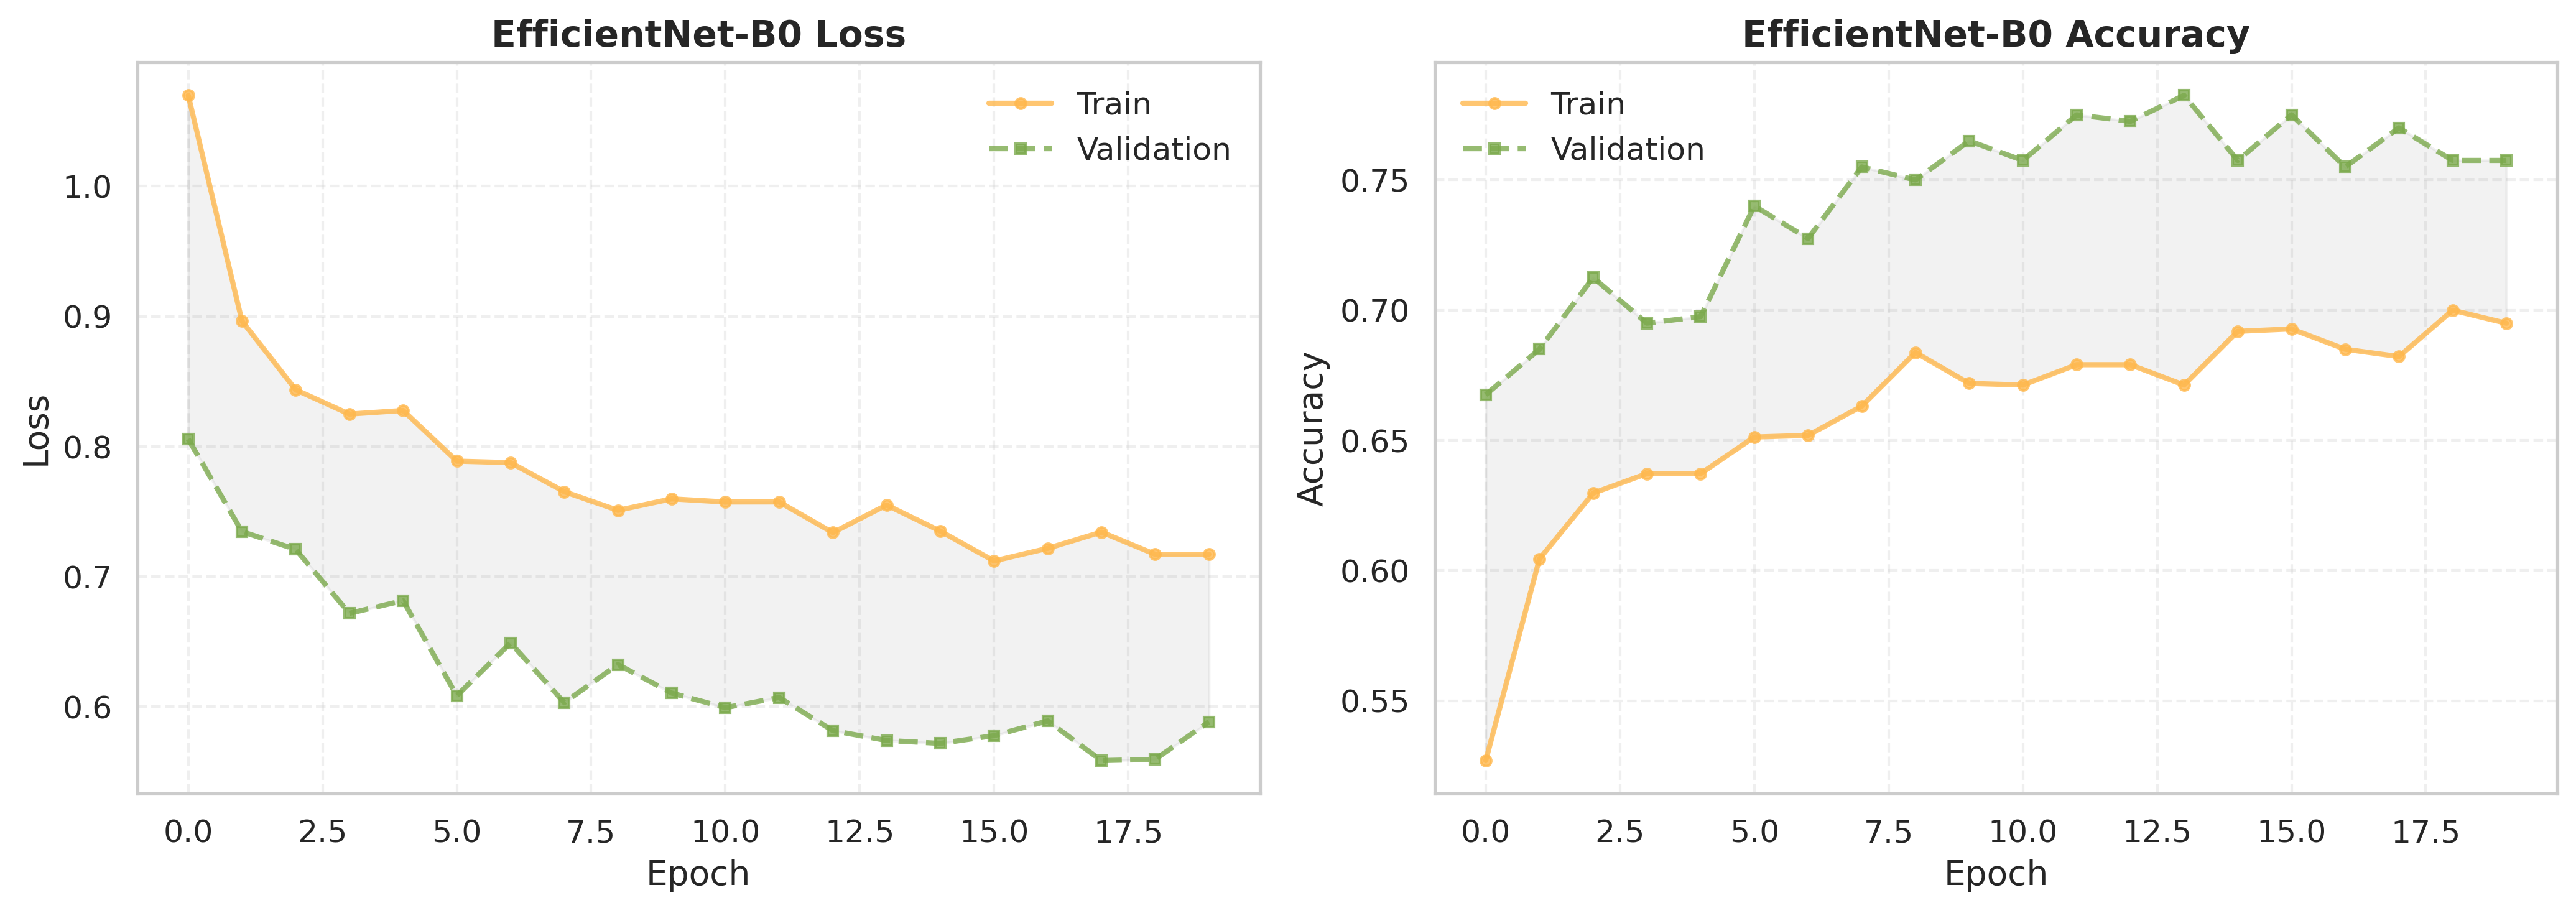
\includegraphics[width=0.8\textwidth]{images/eb.png}
    \caption{Learning curves for \textit{EfficientNet-B0}.}
    \label{fig:eb}
\end{figure*}

\begin{figure*}[!t]
    \centering
    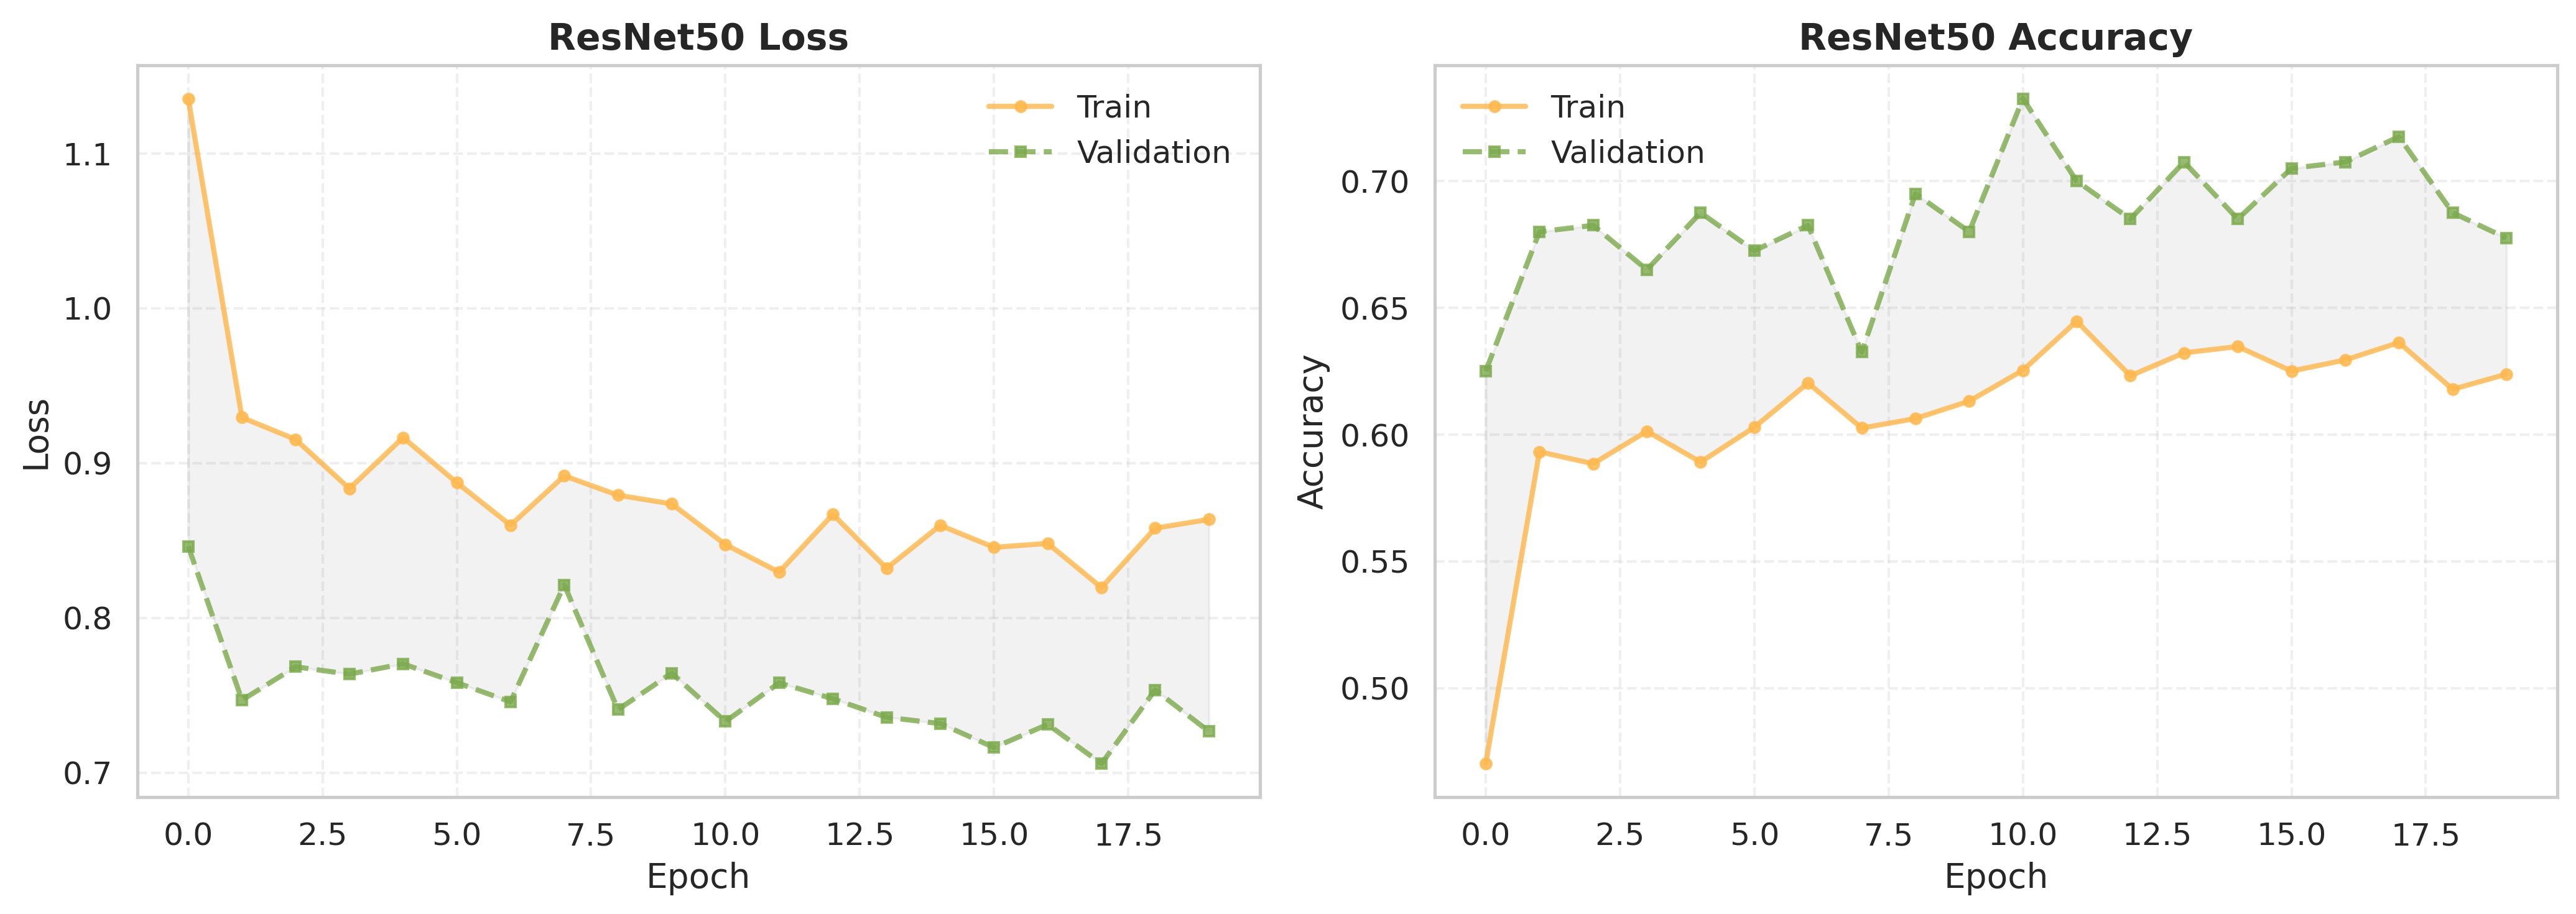
\includegraphics[width=0.8\textwidth]{images/resnet.png}
    \caption{Learning curves for \textit{ResNet50}.}
    \label{fig:resnet}
\end{figure*}

Calss-wise evaluation shows both \textit{EfficientNet-B0} and \textit{ResNet50} showed lower performance on intermediate disease stages; Stage 1 and Stage 2. \textit{EfficientNet-B0} recorded an F1-score of 0.69 for Stage 1 and 0.55 for Stage 2. The \textit{ResNet50} underperformed with F1-scores of 0.57 and 0.51, for Stage 1 and 2 disease. Misclassifications primarily occurred between adjacent disease stages. This limitation was largely mitigated in \textit{SEPierceStageNet} through attention mechanism.

\begin{itemize}
    \item \textbf{\textit{EfficientNet-B0}:} High precision of 0.85 for the Fresh class but lower performance for Stage-2 as F1 recorded 0.55. Had Overall test accuracy of 0.7307.  
    \item \textbf{\textit{ResNet50}:} Moderate precision 0.88 for Fresh but low recall of 0.61. Stage-1 and Stage-2 underperforming. Overall test accuracy was 0.6534.
\end{itemize}
The significant improvement of \textit{SEPierceStageNet} over the baselines: 
\begin{enumerate}
    \item Partial layer freezing to use pretrained features without overfitting dataset.
    \item Integration of attention module to focus on disease specific area of leaf.
    \item Effective classification head tuned for multi-class disease stage differentiation.
\end{enumerate}

These modifications show that carefully designed domain specific models can outperform general-purpose pretrained models in agricultural disease detection tasks.

\section{Limitations and Future Directions}
\label{sec:limitations}

While \textit{SEPierceStageNet} had strong performance in grapevine disease stage classification still several limitations must be acknowledged. And opportunities for improvement still exist. One notable limitation is the dataset size and diversity. The model was trained and evaluated on a dataset of 4004 images which had 401 test samples with predefined disease stages. Although the reported metrics are high, the dataset may not fully contain the variability in grapevine leaves in different climates, lighting conditions, and devices. This can limit the generalizability of the model to different conditions in real-world vineyard scenarios. Additionally, the model exhibits challenges in distinguishing differences between adjacent disease stages, like in Stage 2 and Stage 3. It reflects the difficulty of progressive symptom recognition. Environmental factors also pose a constraint. The current model was trained on images captured under a controlled environment. But on field deployment may bring varying lighting, occlusion by other leaves, dust, or may be overlapping plant structures. All of these can impact prediction accuracy. Although the dataset was balanced across disease stages during training; real world data is often skewed toward early or healthy stages. The performance of \textit{SEPierceStageNet} under such class imbalance conditions remains untested. Despite the inclusion of attention mechanisms that improve feature representation, the model remains a black box and limits interpretability and that hinders real life adoption.

We can address the limitaions by expanding the datasets to include more diverse environmental conditions. Adding multi-modal data like hyperspectral imaging or infrared can improve sensitivity to disease progression and reduce misclassifications between adjacent stages. For practical deployment, developing mobile or edge versions of \textit{SEPierceStageNet} would enable real-time disease detection in-field. Techniques such as focal loss, data augmentation, or synthetic oversampling can help the model remain robust under imbalance data distributions. Integrating interpretability methods such as Grad-CAM, attention heatmaps, or feature attribution can provide visual explanations of predictions and improve trust and usability for agriculture experts. Implementing incremental learning or domain adaptation strategies would allow the model to adapt over time to new disease variants or environmental conditions without full retraining.

In summary, while \textit{SEPierceStageNet} achieves high accuracy in experimental conditions, addressing these limitations will be essential for the practical deployment.


\section{Conclusion}
\label{sec:con}
In this paper, we developed an efficient model for multi-stage classification of grapevine leaves affected by Pierce's disease. The combination of a frozen \textit{EfficientNet-B0} backbone, \ac{se} attention module, and compact classification head gave a better accuracy while keeping computational costs low. Analysis of misclassifications showed that errors were primarily between adjacent stages and the model captures disease progression effectively. The model provides a practical solution for vineyard monitoring, supports early disease detection. Future work will focus on real-world deployment and extension to other grapevine diseases.

\vspace{12pt}
\color{black}

\bibliographystyle{IEEEtran}
\bibliography{references.bib}
\end{document}